\subsubsection{Zel`dovich Pancake}
\label{sec.tests.pancake}

The Zel`dovich pancake \citep{1970A&A.....5...84Z} is particularly
relevant to cosmological simulations, because it includes many
features that are critical to structure formation: hydrodynamics,
expansion, and self gravity.  This problem represents the formation of an ideal,
isolated caustic, and is thus a useful proxy for much more
complicated structures in full 3-dimensional cosmological simulations
(such as the collapse of gas onto a cosmological halo or filament).

The initial conditions are simple, and we follow the prescription of
\citet{Anninos94}.  Assuming a geometrically flat cosmology, the density
perturbation is given by

\begin{equation}
\rho(x_l) = \rho_0 \big[ 1 - \frac{1+z_c}{1+z} \cos(k x_l) \big]
\end{equation}

with the internal energy of the gas set so that the entropy of the gas
maintains a constant value throughout.  The velocity perturbation is given by

\begin{equation}
v(x_l) = -H_0 \frac{1 + z_c}{(1+z)^{1/2}} \frac{\sin(k x_l)}{k}
\end{equation}

In the equations above, $\rho_0$ is the background density, z$_c$ is a
free parameter and is the redshift where the sheet forms a caustic
(i.e., where it `pancakes'), z is the redshift of initialization, x$_l$ is the
Lagrangian mass coordinate, $k = 2 \pi / \lambda$ (where $\lambda$ is
the perturbation wavelength), and H$_0$ is the $z = 0$ value of the
Hubble constant.  Note that this solution is expressed in terms of
Lagrangian positions, so one needs to convert this into the Eulerian
coordinates, x$_e$, that are more useful to \enzo:

\begin{equation}
x_e = x_l - \frac{1 + z_c}{1 + z} \frac{\sin(k x_l)}{k}
\end{equation}

We note that the solution described above is exact up to the point of
caustic formation.  In Figure~\ref{fig.pancake}, we show the results
of a test of the adaptive mesh version of \enzo's Zel'dovich Pancake test.  A
one-dimensional box of length $64$~Mpc/h is initialized at z$ = 20$ in
an $\Omega_M = 1$ universe with h$ = 0.5$ and a background temperature
of 100~K, $\rho_0 = \rho_c$.  The simulation is initialized with 64
grid cells, refining by factors of four using criteria based on cell
mass and the presence of shocks, for a maximum of 2 levels (i.e., an
equivalent maximum resolution of 1024 grid cells).  The simulation was
evolved to z$ = 0$ using the PPM hydro method, with the final output
of the calculation being shown in Figure~\ref{fig.pancake}.

Figure~\ref{fig.pancake} shows the key features of this test problem.
The strong shocks and large density gradients are well-resolved, with
density and velocity jumps being well-delineated and at the correct locations.  The key features of
this test problem can be resolved with far fewer cells -- simulations
including a mere 8 cells resolve the key features, as shown in
Sections 3.3.4-3.3.5 of~\citet{1996PhDT........80B} -- but we choose a
higher resolution here for illustrative purposes.

\begin{figure}
\begin{center}
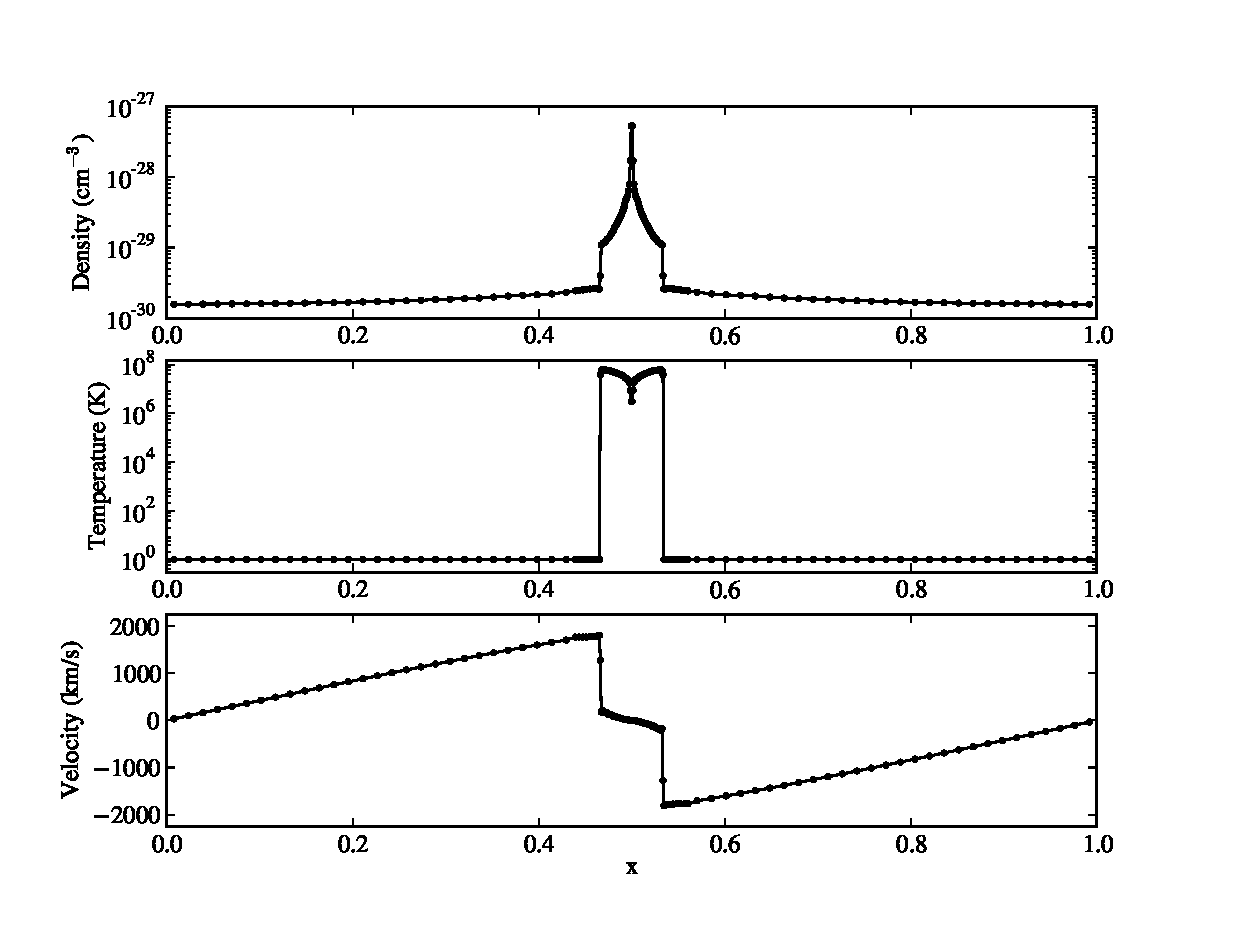
\includegraphics[width=0.8\textwidth]{figures/AMRZeldovichPancake.eps}
\caption{Zel`Dovich Pancake test shown at z$ = 0$, initialized in a
$\Omega_m = 1$ universe at z$ = 20$ on a one-dimensional grid having
64 cells, and further refined by factors of four based on cell mass
and the presence of shocks for up to two additional levels of mesh,
having a maximum effective resolution of 1024 grid cells. The top,
middle, and bottom rows show density, temperature, and velocity of the
gas, respectively; all are a function of position in units of the box
size.  The central region ($x \simeq 0.45-0.55$) has bene adaptively
refined, as can be seen by the locations of grid points.  Shocks and
the central density peak are clearly resolved, with well-delineated
jumps at the appropriate locations.}
\label{fig.pancake}
\end{center}
\end{figure}